\include{template}
\cfoot{} %% if no page number is needed

\begin{document}

\begin{header}
FICHE TECHNIQUE

Dissolution
\end{header}

Quand on mélange un solvant et une espèce chimique pour obtenir une solution, on réalise une dissolution.

\vspace{20pt}
\begin{Large}
\begin{equation}
\color{bleu_f}
C_\mathrm{m}
= \frac{m_\mathrm{soluté}}{V_\mathrm{solution}}
\nonumber
\end{equation}
\end{Large}
\vspace{30pt}

\begin{bframe}
\textbf{Préparation d'une solution par dissolution}
\begin{enumerate}
\item Déterminer la masse de soluté à peser pour réaliser la solution demandée.

\item Préparer la solution.
\end{enumerate}

\begin{multicols}{2}
\paragraph*{Matériel}
\begin{itemize}
\item[•] balance ;
\item[•] coupelle ;
\item[•] entonnoir ;
\item[•] fiole jaugée ;
\item[•] bouchon.
\end{itemize}

\newpage

\paragraph*{Manipulation}
\begin{itemize}
\item[•] Peser le soluté.
\item[•] Mettre le soluté dans la fiole jaugée en rinçant la coupelle et l'entonoir.
\item[•] Remplir la fiole jaugée aux trois-quarts, boucher et agiter.
\item[•] Compléter jusqu'au trait de jauge, boucher et homogénéiser.
\end{itemize}
\end{multicols}

\begin{center}
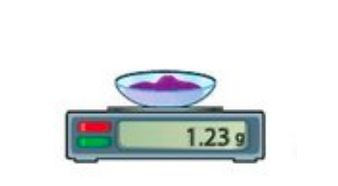
\includegraphics[scale=0.45]{images/pesee.png}
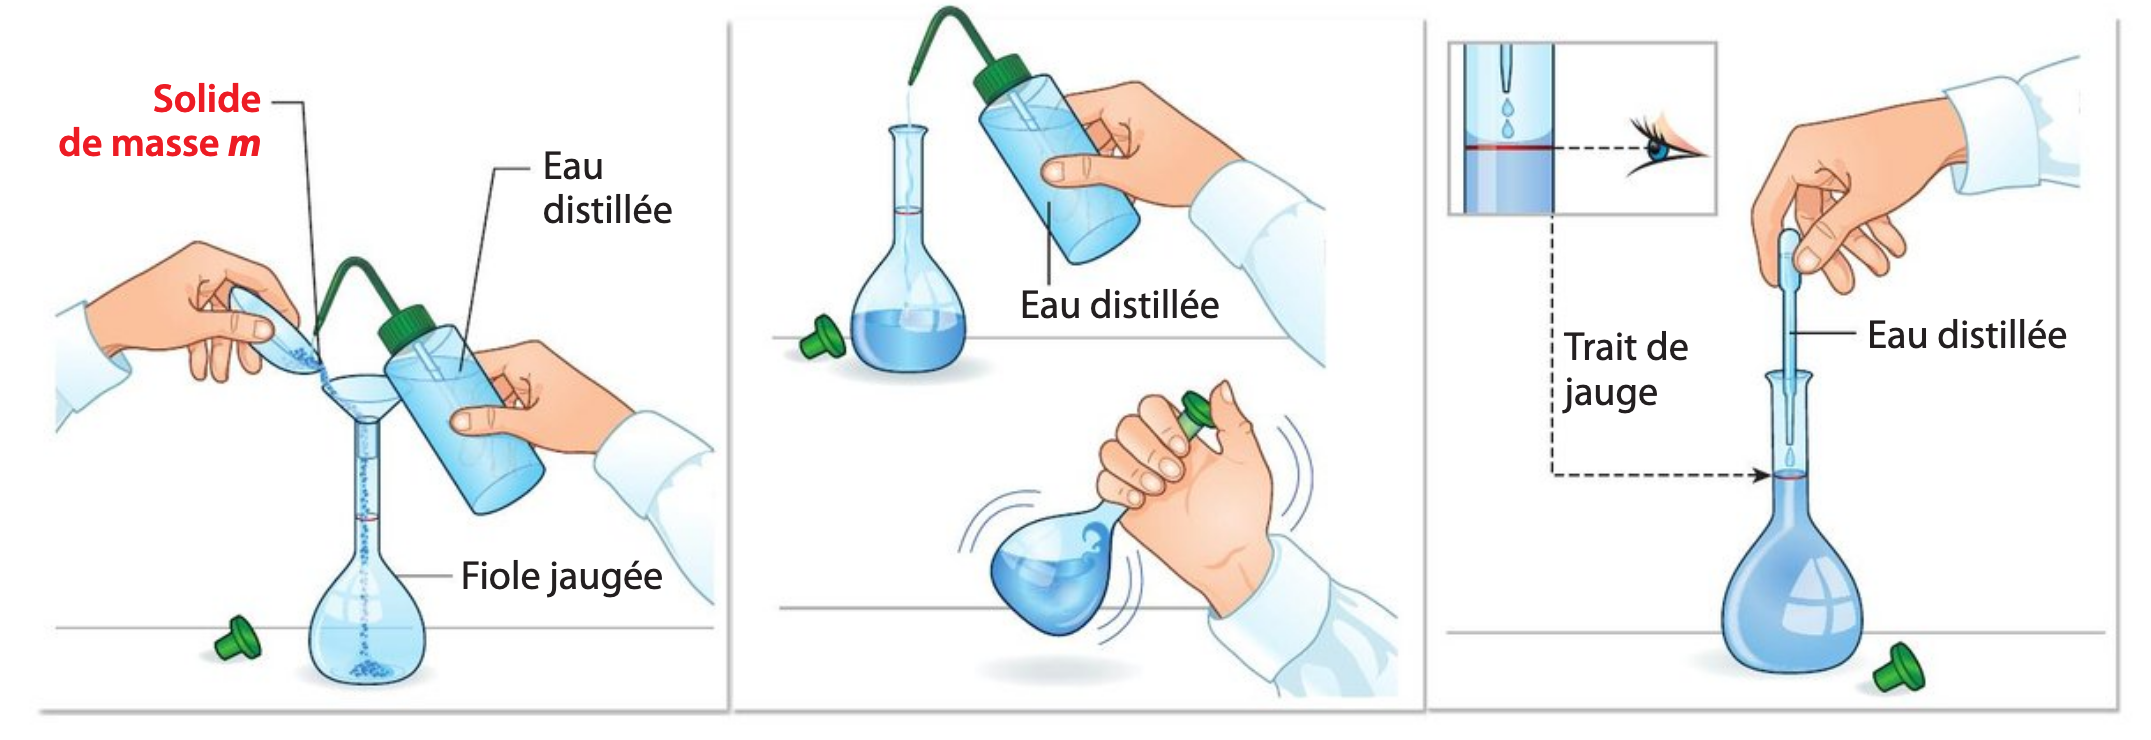
\includegraphics[scale=0.35]{images/dissolution.png}
\end{center}

\end{bframe}

\end{document}